%%
%% Author: shoupu_wan
%% 8/22/18
%%

\chapter{Spiral matrix}\label{ch:spiralMatrix}

\section{The problem statement}\label{sec:ProblemStatement.spiralMatrix}

Depending on the emphasis of the problem, there are several related statements.

\begin{enumerate}
    \item Given two integers $m$ and $n$, generate a matrix of dimension $m \times n$ filled with
    elements from 1 to n2 in spiral order (clockwise, same below).
    \item Give a matrix of dimension $m \times n$, print its the elements in spiral order.
    \item Given a matrix of dimension $m \times n$, starting from the element $M[0][0]$,
    walking down each element in spiral order until all the element has been visited.
    Determine the final element to be visited.
\end{enumerate}

\section{Outline of the algorithm}\label{sec:spiral-matrix-Algorithm}

Unless for some special cases and/or special form of questions,
the algorithm is quite straightforward
\begin{enumerate}[label=\textbf{Step.\arabic*}]
    \label{enum:algorithm}
    \item\label{itm:straight-move} Go straight forward
    and visit each cell in passing as far as possible;
    \item\label{itm:turn-right} When~\ref{itm:straight-move} is not possible
    (facing a wall or visited cell), make a right turn to visit the cell;
    \item\label{itm:goto-terminate} Repeat the above steps until the last cell is visited.
\end{enumerate}

This algorithm is similar to the `wall-follower algorithms' used for solving maze
exploration problems
~\footnote{\url{https://en.wikipedia.org/wiki/Maze_solving_algorithm\#Wall_follower}}.
Interested readers are encouraged to read more in relevant source.

Imagine that the matrix is tightly embedded in a wood frame which serves as the outer wall.
Your goal is to iterate through the matrix elements such that you keep going straight unless
you would revisit a previously visited element or hit the wall.
At which point, make a right turn.
So on and so forth, until you exhaust all the elements.

The key for the solution of this problem is to realize there are two levels of programming.
Firstly, one need to complete one round, peeling off the outermost layer of the matrix and leave
the remaining a smaller matrix.

Secondly, one need to recursively or iteratively loop through the remaining layers.

Once one came up with this insight, coding will be easier and solution will be more readable.

\section{Implementation}\label{sec:spiral-matrix-implementation}

Simple algorithm.
But implementation wise, it could be very verbose and buggy.
Below are some false start.

\subsection{Verbose Implementation}

As mentioned earlier, this problem is a pure coding problem as its algorithm is pretty
straightforward.

Or is it?
In the algorithm ~\ref{itm:straight-move} instructs one to move `straight forward'.
However treacherous complexity is concealed in the two words as there are four directions
for going `straight forward': up, down, left, and right.
The logic of going `straight forward' in each direction is different others.

~\ref{itm:turn-right} in that algorithm, which can be rephrased as `turn right if
you cannot go straight' is equally misleadingly complex---there are four unique turns and each
turn takes unique logic to execute.

Thirdly, spiral motion is subtly different from circular motion in that accompanying each round of
circular motion is \emph{translation motion}.
Particularly in this case, the matrix is gradually `peeled off' as the program execution is
carried out and this `peel off' motion is the extra translational motion.

Last but not least, the problem has a disguised pitfall.
The reader may not have realized but the matrix is not necessarily a square matrix.
Unprepared problem solver would imagine that the program shall terminate right in the
center of the matrix.
But that may not be the case.
For example, for a $2\times n$ matrix, the program would terminate at the `outer layer', while
for $1\times n$ matrix, the matrix reduces to essentially a list and the program would terminate at
the right end.

Dealing these complexities all at once is challenging and prune to bugs.
Even if one succeeds in implementing a working solution, it is doomed to be a mess lacking the
necessary readability and clarity.
\autoref{lst:VerboseSpiralMatrix.java} list an earlier implementation I myself managed to complete.
It works but it is very cumbersome.
If you want to understand what each line of code is doing, I'm sorry, it will take you a while.

\begin{minipage}{\linewidth}
    \lstinputlisting[label={lst:VerboseSpiralMatrix.java},
    caption={Spiral matrix \java implementation.}]
    {case-study/spiral-matrix/VerboseSpiralMatrix.java}
\end{minipage}

\subsection{Analysis of the implementation}

We have provided answer to the `why' question---why implementing this in a more readable way is so
hard.
We are going to illustrate how to come about to implement the
algorithm as stated in ~\autoref{enum:algorithm} in a more readable way.
The key is as mentioned above `dealing these complexities all at once'.
Let's avoid dealing all the complexities at once.
Let's divide up the complexities and conquer them one at a time.
%TODO

This problem is also a coding-focused problem---algorithm is straightforward but if one wants to
code up a neat solution, it'll take a number of skills and effort.

But implementation wise, it's not easy to implement gracefully-free from duplicate code, simple,
and more importantly, easy to read.

But what I found useful is to re-think what can help you close your loop---literally.
\autoref{fig:spiral-matrix-loop}.

\begin{figure}[htb]
    \begin{center}
        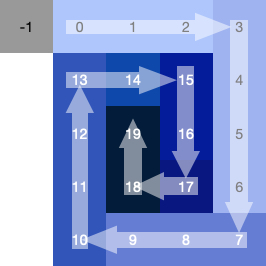
\includegraphics[height=6cm]{case-study/spiral-matrix/spiral-matrix.jpg}
        \caption{An example of applying variational methods to improve an implementation of protobuf
        message visitor pattern.}
        \label{fig:spiral-matrix-loop}
    \end{center}
\end{figure}

\subsection{Recursive implementation}\label{subsec:recursiveImplementation.spiralMatrix}

To simplify the question, one can imagine that the matrix is embedded in a visited

~\autoref{lst:longest_palindromic_substring.py} and \autoref{lst:LongestPalindrom.java} are
implementations in \python and \java, respectively.

\subsection{Spiral Iterator in \python}\label{subsec:spiralIterator}

\begin{minipage}{\linewidth}
    \lstinputlisting[label={lst:spiral_matrix_gen.py},
    caption={Spiral matrix \python implementation.}]
    {case-study/spiral-matrix/spiral_matrix_gen.py}
\end{minipage}
